\subsection{Relativistic Ion Collisions}
Relativistic ion collisions provide experimentalists with a new laboratory for studying QCD.
There are two main classes of collisions that can occur and they are differentiated by the impact parameter ($b$) between the colliding nucleons.
Ultra-peripheral collisions (UPCs) occur when $b>2R_{A}$.
Even though the interacting nuclei do not overlap, a large flux of nearly real photons is present between them.
These photons can interact with each other in light-by-light ($\gamma \gamma$) scattering or with the other nucleus in photonuclear ($\gamma A$) processes.
Hadronic collisions, on the other hand, occur when $b<2R_{A}$.
These collisions are characterized by high multiplicities in the final state.
Hadronic collisions can have sufficient energy and density to briefly form a state of deconfined partonic matter called the Quark-Gluon Plasma (QGP); see Section~\ref{sec:QGP}.
Collisions across these regimes can produce final states ranging from very sparse to high multiplicity.
Experimentally, measuring these collisions is challenging because the environment can be extremely sparse in UPCs or extremely complex in hadronic collisions; both regimes push the limits of detectors.
Since this thesis documents measurements of observables in hadronic nuclear collisions, this section focuses on their properties.
UPCs enter as background to the presented measurements, and steps are taken to remove them from the analysis samples.
\subsubsection{Geometry of Ion Collisions and the Glauber Model}
In a hadronic relativistic ion collision, the two colliding nuclei overlap with some impact parameter $b$.
For simplicity, consider modeling the ions as spheres that are Lorentz-contracted along the beam axis.
In this picture, the ions resemble two flat discs about to collide head-on; see the left panel of Figure~\ref{fig:glauber_schematic}.
\begin{figure}[H]
    \centering
    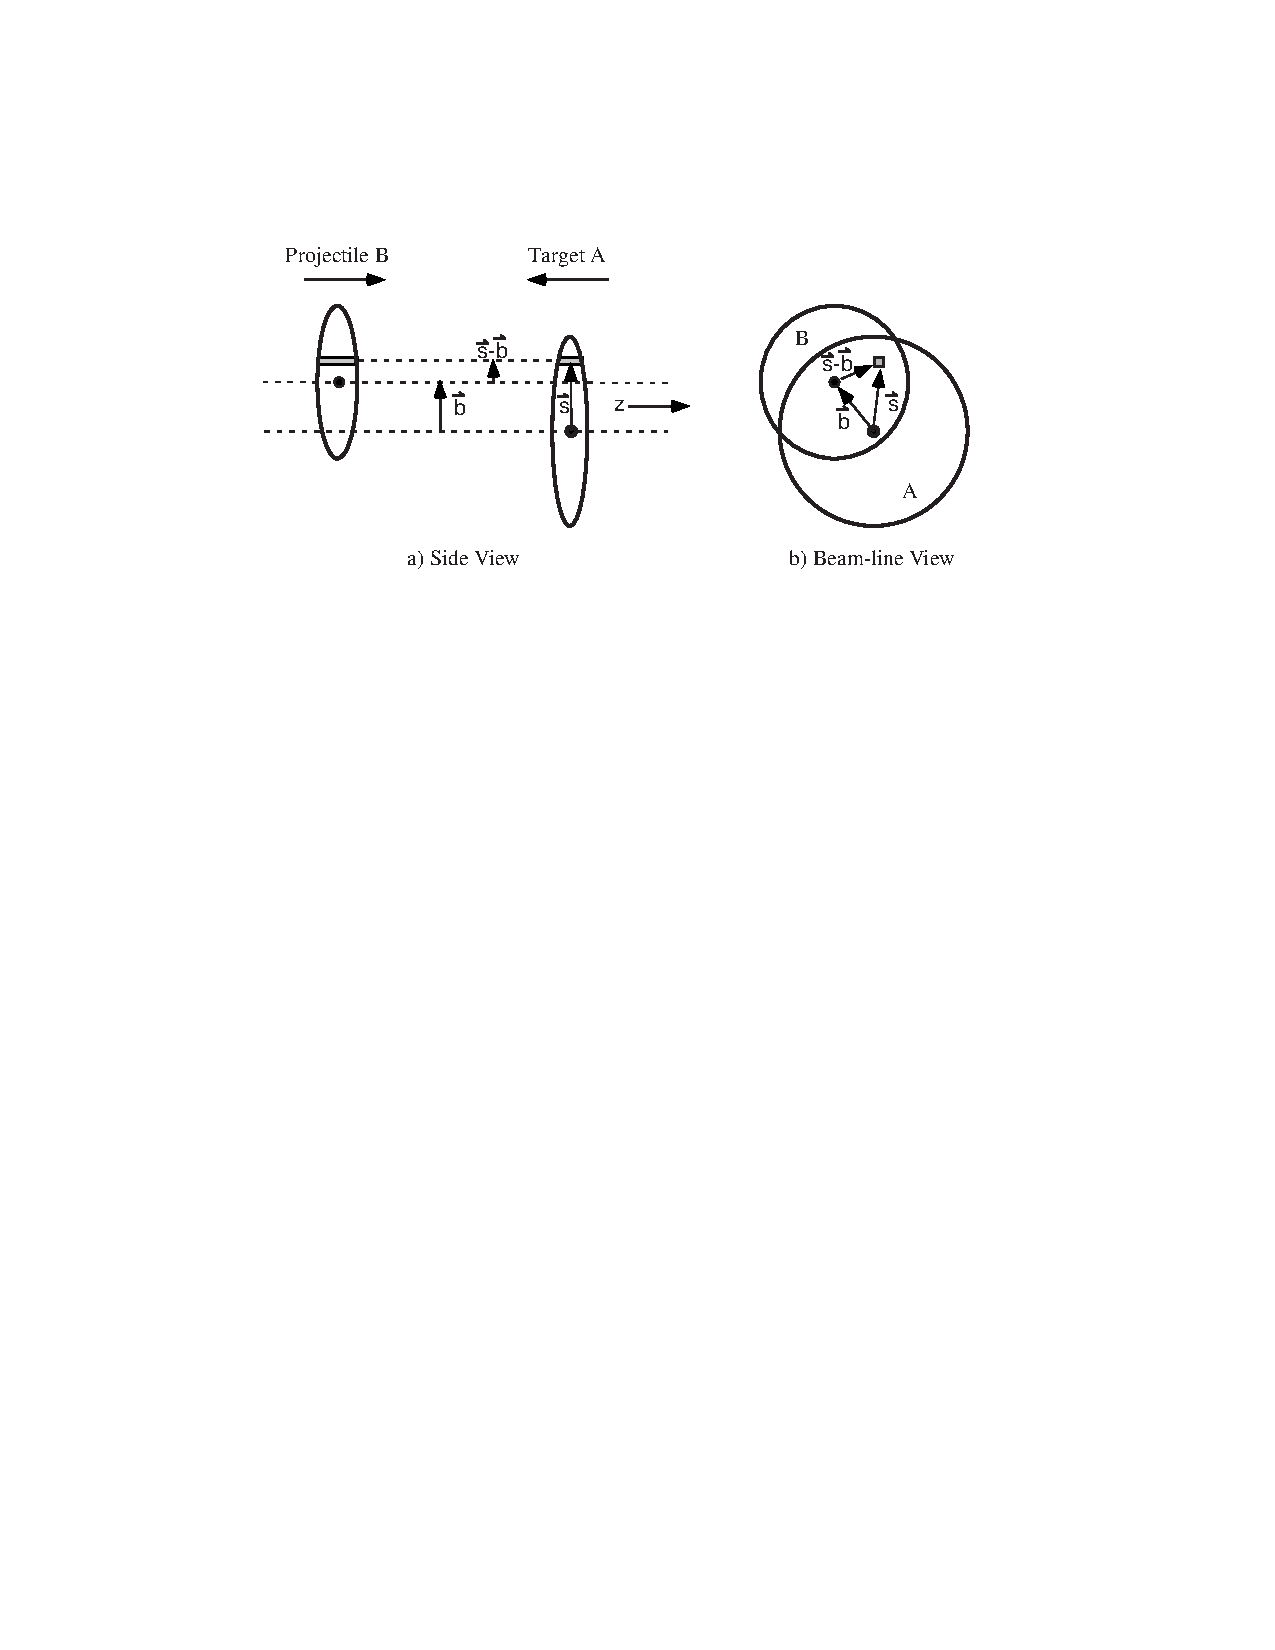
\includegraphics[
        width=0.8\linewidth,
        alt={Schematic illustration of the geometry of a relativistic nuclear collision in the Glauber model.}
    ]{chapters/background/sections/collision_systems/figures/glauberskematic.pdf}
    \caption{Schematic illustration of the ion collision geometry, reproduced from Ref.~\cite{Glauber}.}
    \label{fig:glauber_schematic}
\end{figure}
In this picture, a lower $b$ leads to greater overlap between the two ions.
The greater overlap leads to more nucleon--nucleon interactions and, on average, more final-state particles in the detector.
Figure~\ref{fig:glauber_impact_parameter} compares an O+O collision at $b=2$ fm with a Pb+Pb collision at $b=8$ fm.

This increase in event activity with the initial-state parton flux can be parameterized by the \textit{Glauber model}~\cite{Glauber}.
In its simplest form, the model treats a collision of ions as a superposition of many individual nucleon--nucleon collisions.
Physicists are typically interested in how observables differ from this naive assumption, which provides information about the physics of ion collisions.
The nuclear charge density is typically modeled by a Woods-Saxon distribution:
\begin{equation}
    \label{eq:fermi_distribution}
    \rho(r) = \rho_0\frac{1}{1+\exp{\left(\frac{r-R}{a}\right)}}
\end{equation}
where $\rho_0$ is the central density, $R$ is the nuclear radius, and $a$ is the skin depth.
For the ${}^{208}\mathrm{Pb}$ ion used in this thesis, the values are $R = 6.62 \pm 0.06$ fm and $a = 0.546 \pm 0.01$ fm~\cite{Glauber:PbNuclearRho}.
For the ${}^{16}\mathrm{O}$ and ${}^{20}\mathrm{Ne}$ species used in this thesis, more sophisticated density profiles derived from dedicated quantum Monte Carlo simulations account for correlations between nucleons in small and deformed nuclei~\cite{Glauber:LightIon}.
From the density profiles, one can construct a probability distribution for finding a nucleon at a transverse radius $s$ using Equation~\ref{eq:glauber_TA}.
\begin{equation}
    \label{eq:glauber_TA}
    \hat{T}_A(s) = \int \hat{\rho}_A\left(s,z_A\right)dz_A
\end{equation}
Here, $\hat{\rho}$ is the normalized version of the density in Equation~\ref{eq:fermi_distribution}.
Using these probability distributions, one can construct a joint probability for two nuclear species, A and B. Integrating over this joint probability gives the ``thickness function'' shown in Equation~\ref{eq:glauber_TAB}.
\begin{equation}
    \label{eq:glauber_TAB}
    \hat{T}_{A,B}(b) = \int \hat{T}_A(s)\hat{T}_B(s-b)d^2s
\end{equation}
$\hat{T}_{A,B}(b)$ has units of inverse area. Thus, the probability for a nucleon in ion A to interact with a nucleon in ion B is $\hat{T}_{A,B}(b)\sigma^{\mathrm{NN}}_\mathrm{inel}$, where $\sigma^{\mathrm{NN}}_\mathrm{inel}$ is the inelastic nucleon--nucleon cross section.
Given A nucleons in ion A and B nucleons in ion B, the average number of nucleon--nucleon collisions is given by Equation~\ref{eq:Ncoll}.
\begin{equation}
    \label{eq:Ncoll}
    N_{\mathrm{coll}}(b) = A B \hat{T}_{A,B}(b) \sigma^{\mathrm{NN}}_\mathrm{inel}
\end{equation}
The total number of nucleons participating in the collision is given by Equation~\ref{eq:Npart}.
\begin{equation}
    \label{eq:Npart}
    \begin{aligned}
        N_{\mathrm{part}}(b) ={}& A \int \hat{T}_A(s)\left\{1-\left[1-\hat{T}_B(s-b)\sigma^{\mathrm{NN}}_\mathrm{inel}\right]^{B}\right\}d^2s \\
        &+ B \int \hat{T}_B(s-b)\left\{1-\left[1-\hat{T}_A(s)\sigma^{\mathrm{NN}}_\mathrm{inel}\right]^{B}\right\}d^2s
    \end{aligned}
\end{equation}
Everything discussed so far has implicitly used the ``optical form'' of Glauber theory, which models the nucleus as a sphere with a continuous nucleon density.
This approach allows analytical formulas for $N_{\mathrm{coll}}$ and $N_{\mathrm{part}}$, but it does not describe all features of ion collisions.
The modern approach uses Glauber Monte Carlo.
In this approach, nucleon positions are sampled according to the nuclear density distributions.
If the positions of two nucleons are unphysically close (i.e. almost on top of one another) the position for one of them is redrawn.
Next, a random impact parameter is drawn, and the colliding nuclei are placed accordingly.
The nucleons at their sampled positions in A and B travel along straight-line trajectories.
If two nucleons from the colliding ions come closer than $\sqrt{\sigma^{\mathrm{NN}}_\mathrm{inel}/\pi}$ along these paths, they are considered to have undergone a nucleon--nucleon collision, and $N_{\mathrm{coll}}$ is incremented by one.
The Monte Carlo approach can be thought of as a summation of these individual collisions, where any nucleon that enters one contributes to $N_{\mathrm{part}}$.
From many Monte Carlo events, one can build distributions of $N_{\mathrm{coll}}$ and $N_{\mathrm{part}}$, from which the averages $\langle N_{\mathrm{coll}} \rangle$ and $\langle N_{\mathrm{part}} \rangle$ are extracted.
The optical and Monte Carlo approaches tend to differ most in situations where fluctuations in nucleon positions are important, such as in simulations of light ions or large-$b$ heavy-ion collisions.
Single event Glauber Monte Carlo profiles for \OxO\ and \PbxPb\ collisions are shown in Figure~\ref{fig:glauber_impact_parameter}.

\begin{figure}[H]
    \centering
    \begin{subfigure}[t]{0.49\linewidth}
        \centering
        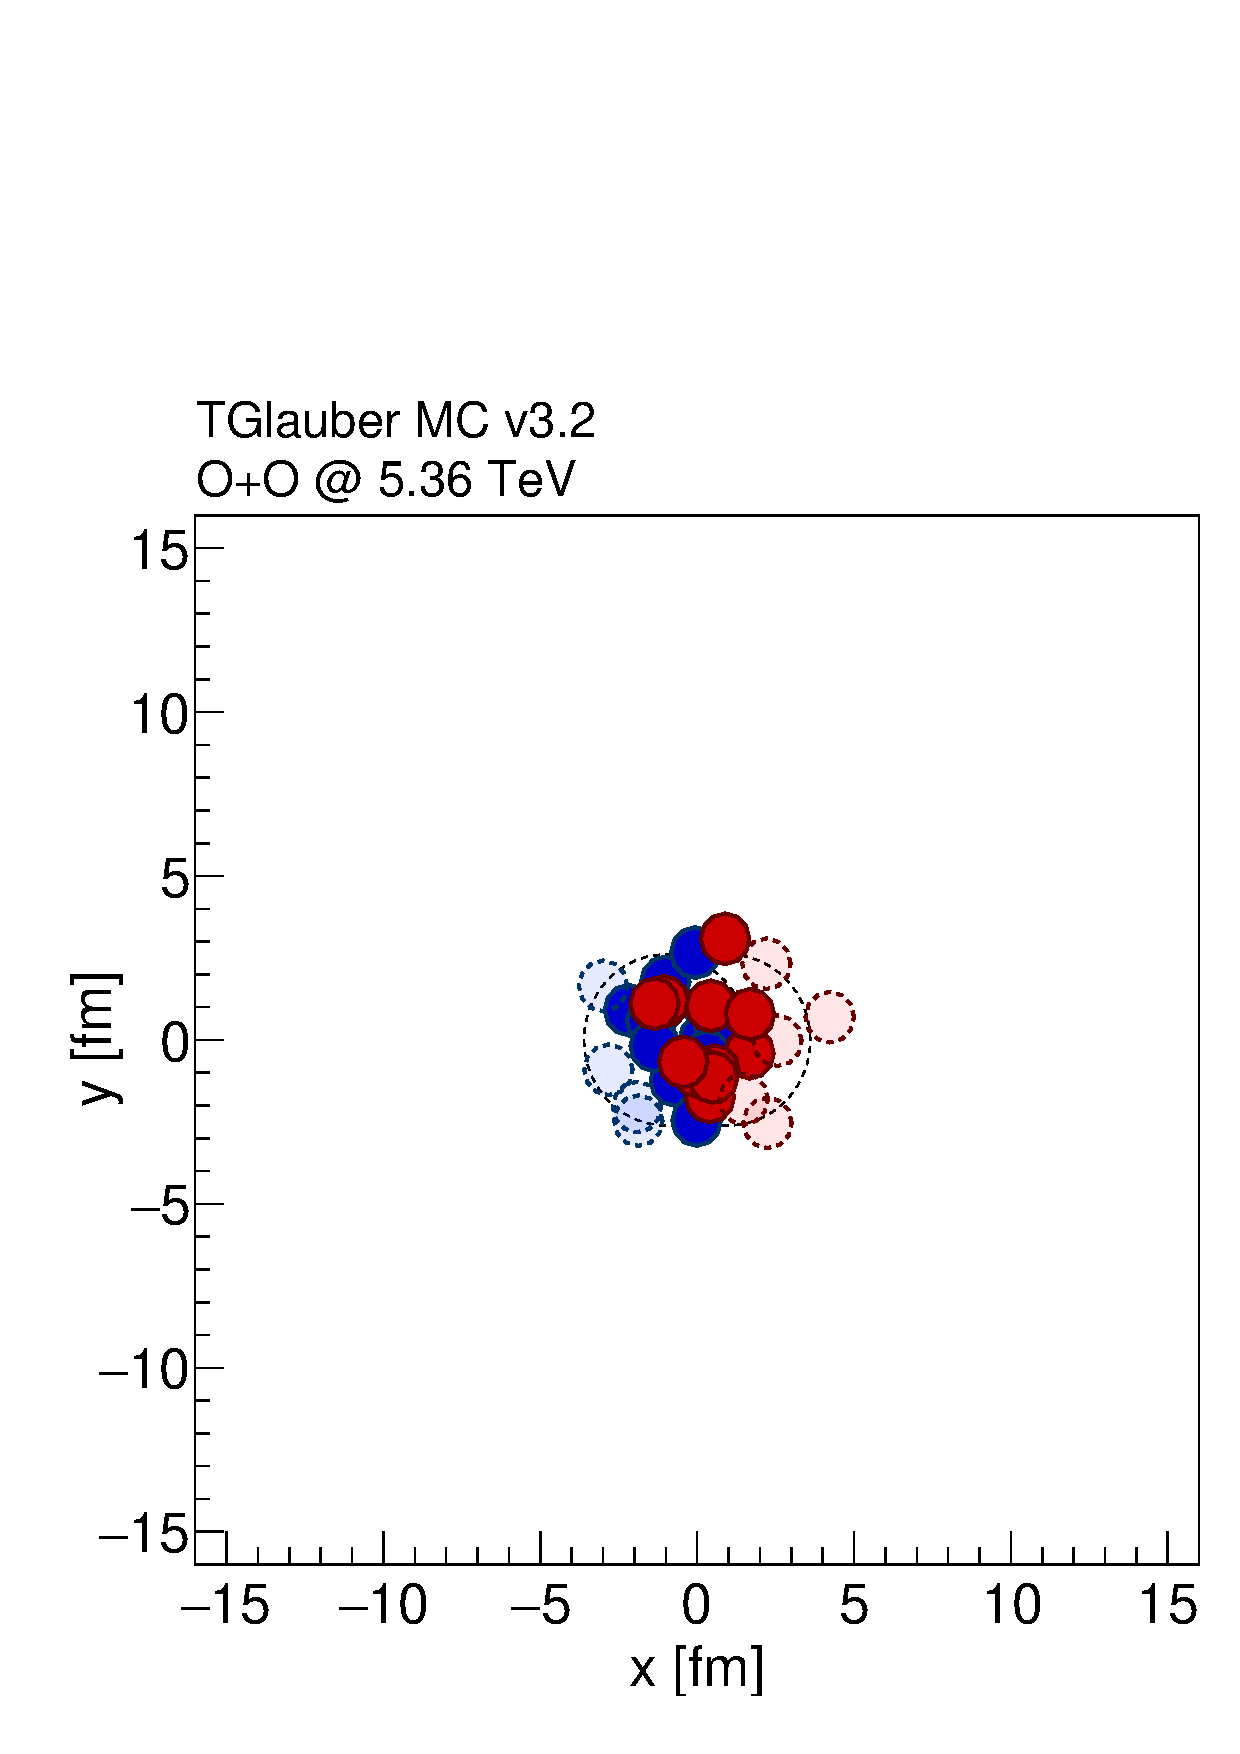
\includegraphics[
            width=\linewidth,
            alt={Schematic of an oxygen-oxygen collision at an impact parameter of 2 femtometers.}
        ]{chapters/background/sections/collision_systems/figures/OO_b2fm.pdf}
    \end{subfigure}
    \hfill
    \begin{subfigure}[t]{0.49\linewidth}
        \centering
        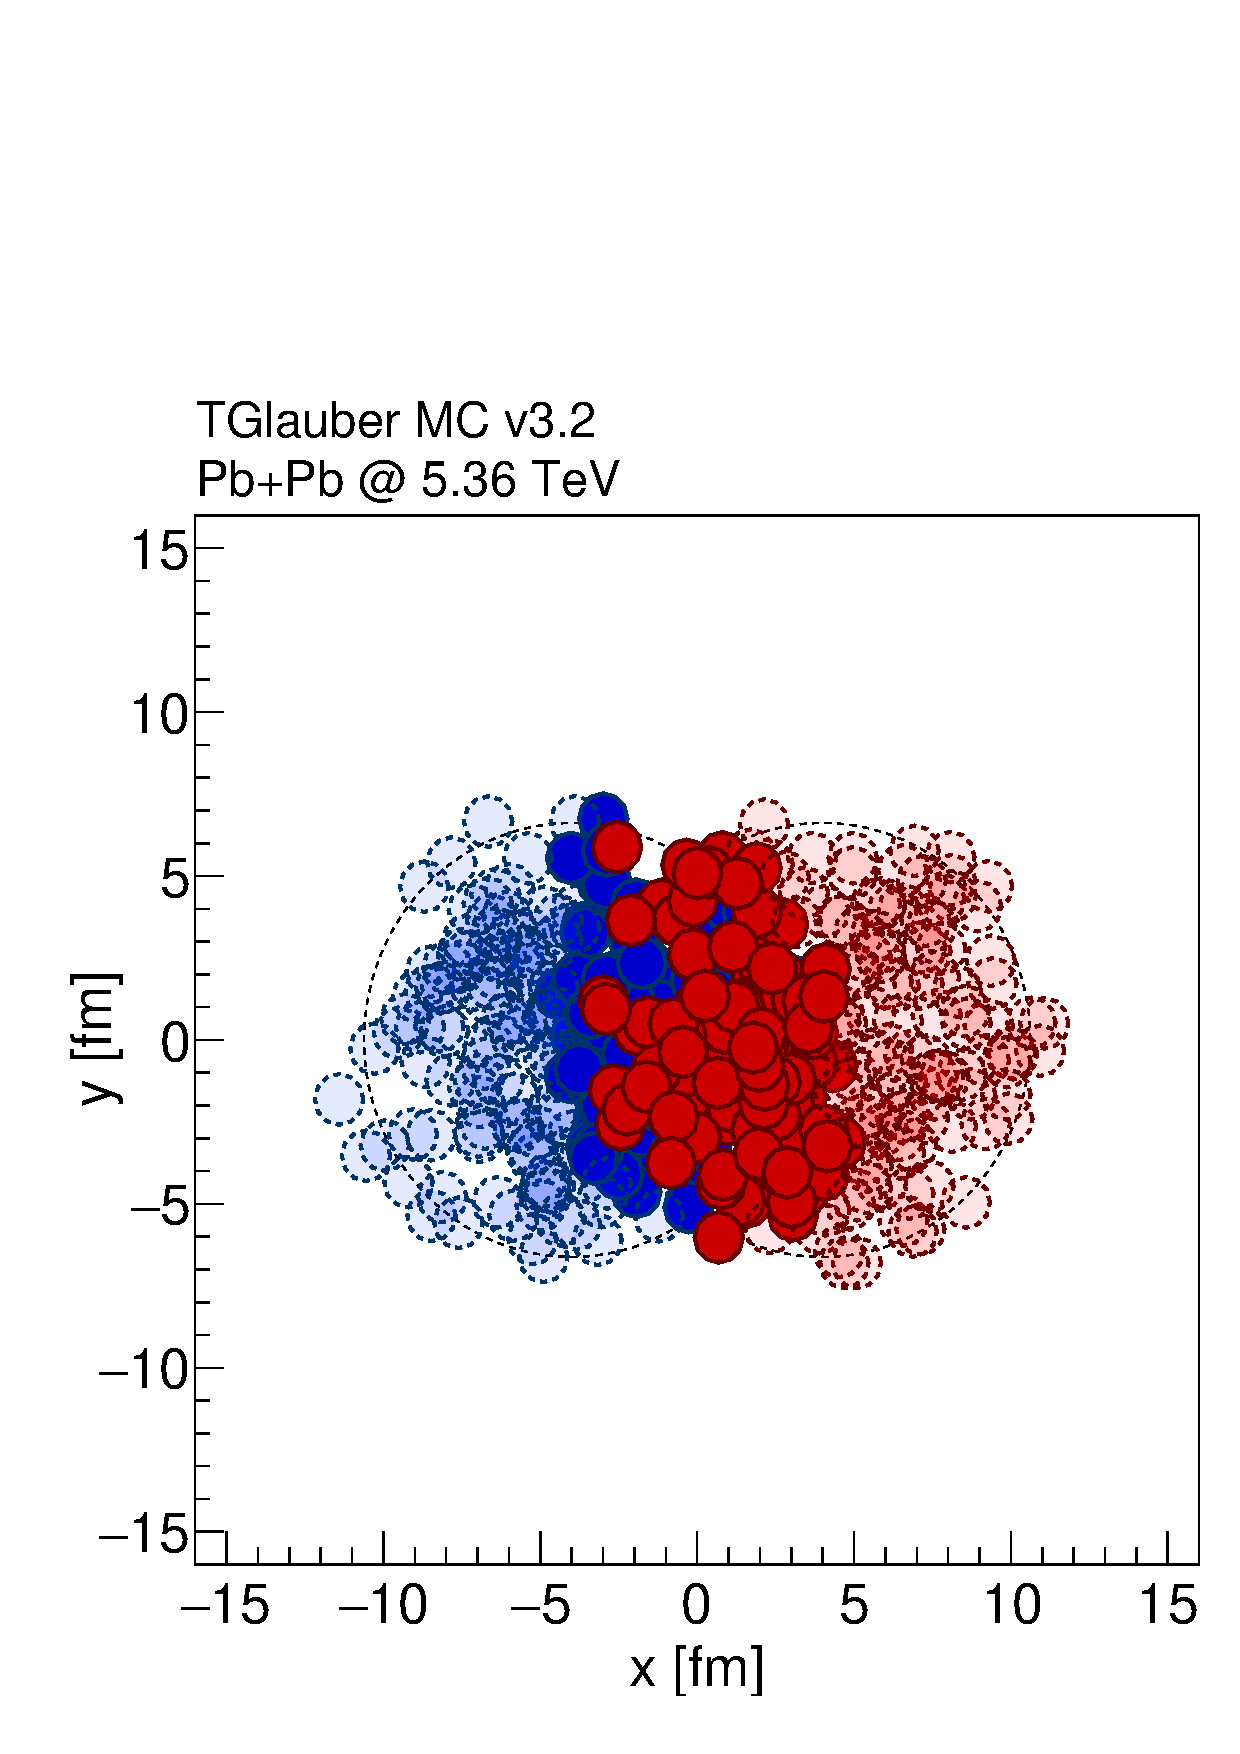
\includegraphics[
            width=\linewidth,
            alt={Schematic of a lead-lead collision at an impact parameter of 8 femtometers.}
        ]{chapters/background/sections/collision_systems/figures/PbPb_b8fm-1.pdf}
    \end{subfigure}
    \caption{Distributions of nucleons generated with Glauber Monte Carlo in the $x--y$ transvrse plane. The two nuclei are shown in different colors, with the particiapents shown as darker circules. Results for \OxO\ collisions (left) and \PbxPb\ collisions (right) are shown. Figures provided by R. Longo.}
    \label{fig:glauber_impact_parameter}
\end{figure}

Since the impact parameter between colliding nuclei is not experimentally accessible, one needs some type of modeling to connect the impact parameter to something measurable.
This is typically done through so-called ``global observables'' like forward transverse energy or charged particle multiplicity, which are thought to be monotonically related to $b$.
The mapping between impact parameter in a Glauber simulation and the global observable is given by a \textit{centrality} calibration; this is why these global observables are also referred to as \textit{centrality estimators} (CE).
Additionally, the data used as input to these centrality calibrations consist of minimum-bias inelastic collisions.

The two-component model is used for the measurements presented in this thesis.
This model postulates that the CE in ion collisions scales with the effective number of \textit{production elements}.
\begin{equation}
    N_{\mathrm{elem}} = xN_{\mathrm{coll}}+ (1-x) N_{\mathrm{part}}/2
\end{equation}
where $x \in \left(0,1\right)$.
First, a distribution of the CE is fit to \pxp\ data, which represents $N_{\mathrm{elem}}=1$.
Then, the CE distribution in ion collisions can be modeled as an $N_{\mathrm{elem}}$-fold convolution of the \pxp\ fit, with the distribution of $N_{\mathrm{elem}}$ obtained from the Glauber Monte Carlo.
The templated ion Monte Carlo CE distribution is then fit to the corresponding distribution in ion data, which is histogrammed above a low CE threshold.
This threshold represents the lowest CE value for which a contribution from UPC events can be neglected, so that the centrality calibration corresponds only to hadronic collisions.
The free parameters in this fit are the $x$ in the $N_{\mathrm{elem}}$ extraction, and the specific fit parameters for the single element CE extraction which were initialized on \pxp\ data.
Once the ion Monte Carlo CE fit has converged, typically to a value of $x\approx0.1$, the fraction of the total hadronic cross section sampled by the experiment, $f_{\mathrm{samp}}$, can be extracted.
This is done by looking at the fraction of the ion Monte Carlo CE distribution above the low CE threshold; typical values are $f_{\mathrm{samp}} \approx 0.8\%$.
The centrality percentiles can then be extracted from the data by dividing it into $f_{\mathrm{samp}} \times 100$ equal-sized percentile bins.
Centrality percentiles are defined such that low percentiles correspond to collisions with large parton flux (low $b$), typically called \textit{central collisions}, while high percentiles correspond to collisions with low parton flux (high $b$), typically called \textit{peripheral collisions}.
The most central percentile bin is $\left[0\%,1\%\right]$, corresponding to the highest CE values. The most peripheral percentile bin is $\left[f_{\mathrm{samp}} \times 100 - 1 \;\%, f_{\mathrm{samp}} \times 100\;\%\right]$, corresponding to the lowest CE values measured above the low threshold.
Once these bins have been defined, the $\langle N_{\mathrm{coll}} \rangle_{\mathrm{bin}}$, $\langle N_{\mathrm{part}} \rangle_{\mathrm{bin}}$, and $\langle T_{A,B}\rangle_{\mathrm{bin}}$ can be extracted per-bin.
In this way, subsets of the experimental data can be associated with geometric quantities from Glauber modeling, and observables can be studied as a function of centrality.
\subsubsection{\texorpdfstring{Control Systems: $pp$ and $p$+A collisions}{Control Systems: pp and p+A collisions}}
Reletvistic ion collisions are primarily oriented towards the goal of studying the QGP.
To isolate the effects of the QGP, it is often the case than an obervable is measured in \AxA\ collisions and also in a control system.

It is an open question if any (or how much) QGP is produced in control systems.
This topic will be discussed more later in Sction~\ref{sec:qgp_small}.
For this broad introduction, it is sufficient to note that any QGP formed in \pxp\ or \pxA\ collisions is expected to be small enough that its effects on many final-state observables are limited.
These observables can often be described well by theoretical models that do not include QGP effects.
The above statement is often not true for \AxA\ collisions, which is why we can say that \pxp\ and \pxA\ systems can be used as control systems.
Additinally, systems colliding a very large and very small ion, like \dxAu\ collisions at the Reletivistic Heavy Ion Collider (RHIC), also behave as control systems for the same reason.

\pxA\ collisions can be very useful to study nPDF effects coming from the A nucleus.
Cross sectional measurments perfomred in \pxA\ collisions can directly constrain the nPDFs.
These constraints improve predictions for \AxA\ measurements and help disentangle QGP effects from potentially substantial nPDF effects.

\subsubsection{\texorpdfstring{Centrality biases from color transparency in $p$+A collisions}{Centrality biases from color transparency in p+A collisions}}
Centrality can be defined in \pxA\ collisions in a similar way to \AxA\ collisions.
As the projectile (proton) impacts the target (ion) at different impact parameters it will on avergae encounter fewer target nucleons at high-$b$ than it will at low-$b$.
This creates the normal scaling we expect, where the CE scales invserly with the impact paramter.
A key feature of \pxA\ collisions is the asymmetry of the incoming system: a single proton collides with a nucleus.
As the proton traverses the nucleus, successive nucleon--nucleon interactions can reduce its available energy.
Meanwhile, target nucleons that have not yet interacted retain their beam energy, contributing to a net energy-flow imbalance toward the target direction.
This means that measurments of CE are typically restricted to the nucleus-going direction, as the proton-going energy flow is less corralated with $N_{\mathrm{elem}}$.

The Glauber Monte Carlo can be run for \pxA\ in much the same way it was for \AxA.
Here the relationship between $N_{\mathrm{coll}}$ and $N_{\mathrm{part}}$ is trivial $N_{\mathrm{coll}} = N_{\mathrm{part}} -1$.

However, impact parameter is not the only variable that impacts the $N_{\mathrm{coll}}$.
As discussed in Section~\ref{sec:CT}, color transparency effects impact the interaction strength of the proton, leading to fewer wounded nucleons in the same target nucleus, all else being equal, as shown in Figure~\ref{fig:color_fluctuation_pA}.  The impact on $N_{\mathrm{coll}}$ is exactly the same as if the event was more periphiphral than it really is.
This leads to a systematic bias, when events are partitioned in both centrality and some quantity that can be mapped onto the Bjorken-$x$ of the proton\footnote{For example jet \PT\ and $\eta$.}.

\TCR{Introduce Aric measurment here or before paper?}

\subsubsection{Luminosity}

\TCR{Placeholder text for Luminosity}
